\chapter{随机热机}
\section{随机热力学}

\section{随机热机模型}

\section{绝热捷径}
\qquad 在有限时间热力学中,一个非常重要的议题是如何实现不同平衡态的相互转换。因为\textbf{有限时间}的限制使得我们不能够使用准静态的方法,而绝热捷径\cite{Chen2010}提供了这样一种可以在有限时间内实现平衡态转化的策略。这个策略是由 Demirplak and Rice \cite{Demirplak2003}和 Berry \cite{Berry2009} 独立发展出来的。\R{(两篇文章相隔太久,很奇怪,出自\cite{Jarzynski2013})}在这个策略发展处以后的很长一段时间内,它引起了一大批研究者的关注。下面我们回顾一下绝热捷径是怎么实现的。

考虑量子力学中的绝热定理\cite{Griffiths2018}:如果一个系统的哈密顿量$H_0(t)$随时间变化很缓慢,即$\tau_\mathrm{e} \gg \tau_\mathrm{i}$,其中$\tau_\mathrm{e}, \tau_\mathrm{i}$分别表示环境的特征时间和系统的内部特征时间。那么如果系统在时间$t=0$处于$H_0 (0)$的本征态,即系统的初态$| \psi(0) \rangle = | n(0) \rangle$,绝热定理告诉我们系统在$t$时刻会处于$H_0 (t)$的对应于瞬时本征态$| n(0) \rangle$,并且
\begin{equation}
    |\psi(t)\rangle=|n(t)\rangle e^{i \theta_{n}(t)} e^{i \gamma_{n}(t)}
    \label{eq2.1}
\end{equation}

其中$\theta_{n}(t)=-\frac{1}{\hbar} \int_{0}^{t} E_{n}(t^{\prime}) \M{d} t^{\prime}, \gamma_{n}(t)=i \int_{0}^{t}\langle n(t^{\prime}) | \partial_{t^{\prime}}n(t^{\prime})\rangle \M{d} t^{\prime}$

不难注意到,绝热定理实现了$H_0(t)$的对应的本征态之间的转化$| n(0) \rangle \to | n(t) \rangle$。现在我们考虑取消$\tau_\mathrm{e} \gg \tau_\mathrm{i}$的要求。

假设存在一个哈密顿量$H(t)$,它使得系统的态的演化严格为$|\psi(t)\rangle=|n(t)\rangle e^{i \theta_{n}(t)} e^{i \gamma_{n}(t)}$,则根据薛定谔方程有
\begin{equation}
    i \hbar \PP{}{t} |\psi(t)\rangle= H(t) |\psi(t)\rangle
    \label{eq2.2}
\end{equation}

将\ref{eq2.1}代入\ref{eq2.2},整理得$ E_{n}+ i \hbar \left( | \partial_{t} n \rangle -\langle n | \partial_t n \rangle\right)|n\rangle=H| n\rangle$,于是可得
\begin{align}
    \nonumber H(t)&=H_{0}(t)+i \hbar \sum_{m}\left(\left|\partial_{t} m\right\rangle\left\langle m\left|-\left\langle m \mid \partial_{t} m\right\rangle\right| m\right\rangle\langle m|\right) \\
    &\equiv H_0 + H_1
    \label{eq2.3} 
\end{align}

于是一个以$H (t)$作为哈密顿量的系统,若其初态为$H_0 (t)$的本征态$| n(0) \rangle$,那么不论$H (t)$随时间的变化快慢与否,在$t$时刻,系统的状态依然是$H_0 (t)$的本征态,只是两者有一个相位差。于是我们实现了在有限时间内的本征态之间的转化。这其中的关键在于我们引进了一个\textbf{反绝热哈密顿量}$H_1 (t)$,根据\ref{eq2.3},我们已经在形式上得到了$H_1 (t)$。现在我们考虑对于具体的$H_0 (t)$,如何得到$H_1 (t)$的具体表达式。\cite{Jarzynski2013}

让$H_0$通过一系列参数$\bm{\lambda}(t)=\left( \lambda_1 (t) , \lambda_1 (t) , \lambda_1 (t) , \cdot , \lambda_{N} (t) \right)$依赖于时间$t$。同时,$H_0 (\bm{\lambda})$的本征值、本征态为$E_n (\bm{\lambda}), | n (\bm{\lambda}) \rangle$,根据复合函数的微分法则,式\ref{eq2.4}可以写为
\begin{equation}
    H_1 (t)=\dot{\boldsymbol{\lambda}} \cdot \boldsymbol{\xi}(\boldsymbol{\lambda}(t))
    \label{eq2.5}
\end{equation}
其中
\begin{equation}
    \boldsymbol{\xi}(\boldsymbol{\lambda})=i \hbar \sum_{m}(|\boldsymbol{\nabla} m\rangle\langle m|-\langle m \mid \boldsymbol{\nabla} m\rangle| m\rangle\langle m|)
    \label{eq2.4}
\end{equation}
同时$|\nabla m\rangle \equiv \partial_{\boldsymbol{\lambda}}|m(\boldsymbol{\lambda})\rangle  , \dot{\boldsymbol{\lambda}} \equiv \mathrm{d} \lambda / \mathrm{d} t$

把$\boldsymbol{\xi}$看做参数空间的无穷小平移$\boldsymbol{\lambda} \to \boldsymbol{\lambda} + \delta \boldsymbol{\lambda}$的生成元。这个无穷小平移与希尔伯特空间中态的变换$|\psi\rangle \rightarrow|\psi\rangle+|\delta \psi\rangle$相联系,通过以下方式
\begin{equation}
    i \hbar|\delta \psi\rangle=\delta \boldsymbol{\lambda} \cdot \boldsymbol{\xi}|\psi\rangle
    \label{eq2.6}
\end{equation}
这样,在一阶近似下,$H_0 (\bm{\lambda})$的本征态$|n(\bm{\lambda})\rangle$的变换为\R{(有一点不懂,额外的相位怎么出来的\cite{Jarzynski2013})}
\begin{equation}
    |n(\boldsymbol{\lambda})\rangle \rightarrow\left(1+\frac{1}{i \hbar} \delta \boldsymbol{\lambda} \cdot \hat{\boldsymbol{\xi}}\right)|n(\boldsymbol{\lambda})\rangle=e^{i \delta \boldsymbol{\lambda} \cdot \boldsymbol{A}_{n}}|n(\boldsymbol{\lambda}+\delta \boldsymbol{\lambda})\rangle
    \label{eq2.7}
\end{equation}
其中$\boldsymbol{A}_{n}(\boldsymbol{\lambda})=i\langle n | \boldsymbol{\nabla} n\rangle.$ 这意味着,沿着参数空间的曲线$\bm{\lambda}$利用式\ref{eq2.7},可以将系统的态逐步从$|n(\M{\lambda_0})\rangle$变换成$\M{e}^{i \int_{\bm{\lambda_0}}^{\bm{\lambda_s}}   i\langle n | \boldsymbol{\nabla} n\rangle \M{d}\bm{\lambda}}\left|n\left(\boldsymbol{\lambda}_{s}\right)\right\rangle.$ 这正是们所希望得到的形式。

现在看看系统态的时间演化,先考虑系统经过一个无穷小时间$\delta t$,则态$|\psi \rangle$将演化为
\begin{equation}
     \left(1+\frac{1}{i \hbar} H \delta t\right)|\psi\rangle=|\psi\rangle+\frac{1}{i \hbar} \delta t H_{0}|\psi\rangle+\frac{1}{i \hbar} \delta \boldsymbol{\lambda} \cdot \boldsymbol{\xi}|\psi\rangle
   \label{eq2.8}
\end{equation}

如果考虑态$|\psi \rangle = |n(\bm{\lambda}) \rangle$,那么\ref{eq2.8}的物理意义是明显的。$H_0$产生了我们熟悉的动力学相位,而$\boldsymbol{\xi}$产生了几何相因子。

由\ref{eq2.4}定义的$\bm{\xi}$,也可由下式\ref{eq2.9}定义,(二者的等价性可由$\langle m \mid \boldsymbol{\nabla} n\rangle=\left\langle m\left|\boldsymbol{\nabla} \hat{H}_{0}\right| n\right\rangle /\left(E_{n}-E_{m}\right)$\cite{Berry2009}加以证明)
\begin{subequations}
    \begin{align}
        \left[ \boldsymbol{\xi}, H_{0} \right] &= i \hbar \left( \boldsymbol{\nabla} H_{0}-\operatorname{diag} \left(\boldsymbol{\nabla} H_{0} \right) \right) \label{eq2.9a}\\
        \langle n|\boldsymbol{\xi}| n\rangle &= 0 \label{eq2.9b}
    \end{align}
    \label{eq2.9}
\end{subequations}
其中$\operatorname{diag}\left(\boldsymbol{\nabla} H_{0}\right)=\sum_{m}|m\rangle\left\langle m\left|\boldsymbol{\nabla} H_{0}\right| m\right\rangle\langle m|.$ 对\ref{eq2.9a}两端同时进行操作$\langle m|\cdots| n\rangle$,得到$\langle m| \boldsymbol{\xi} | n\rangle (E_n - E_m) = \langle m|i \hbar \left( \boldsymbol{\nabla} H_{0}-\operatorname{diag} \left(\boldsymbol{\nabla} H_{0} \right) \right)| n\rangle$. 可见,\ref{eq2.9a}决定了$\boldsymbol{\xi}$的非对角元,\ref{eq2.9b}决定了其非对角元。

式\ref{eq2.9}提供了一种在经典力学中找到\textbf{反绝热哈密顿量}的对应方法。因为我可以利用量子与经典的对应$[A, B]/i \hbar \to \{A, B\}  $将\ref{eq2.9}转换为经典的,进而可以在经典力学中找到对应的\textbf{反绝热哈密顿量}。现在考虑一个经典系统,其自由度为1,哈密顿量为$H_0 (\bm{\eta};\bm{\lambda}).$ 其中$\bm{\lambda}$依然为依赖于时间的一系列参数,$\bm{\eta}=(q,p)$为广义坐标和广义动量,确定了相空间的一个点。对于确定的能量$E = H_0 (\bm{\eta};\bm{\lambda})$,这将相点约束在相空间的一个能壳上,积分
\begin{equation}
    I(E, \boldsymbol{\lambda}) \equiv \int \mathrm{d} \bm{\eta} \theta\left[E-H_{0}(z ; \boldsymbol{\lambda})\right]
  \label{eq2.10}
\end{equation}
表示的是能壳所围成的体积,阶跃函数$\theta\left[E-H_{0}(z ; \boldsymbol{\lambda})\right]$可以使得积分区域为整个相空间。经典的绝热定理告诉我们$I(E, \boldsymbol{\lambda})$是一个\textbf{绝热不变量}\cite{LiuChuan2019}。也就是说如果$H_0$随时间$t$变化的足够缓慢,那么能壳所围成的体积将保持不变。定义任意可观测量$A$的\textbf{微正则分布平均}
\begin{equation}
    \langle A \rangle_{E, \lambda} \equiv \frac{1}{\partial_{E} I} \int \mathrm{d} \bm{\eta} \delta\left(E-H_{0}\right) A
  \label{eq2.11}
\end{equation}
利用函数$I (E,\bm{\lambda})$去定义函数$E (I, \bm{\lambda})$,则有
\begin{equation}
    \boldsymbol{\nabla} E(I, \boldsymbol{\lambda})=-\frac{\boldsymbol{\nabla} I(E, \boldsymbol{\lambda})}{\partial_{E} I(E, \boldsymbol{\lambda})}=\left\langle\boldsymbol{\nabla} H_{0}\right\rangle_{E, \boldsymbol{\lambda}}
  \label{eq2.12}
\end{equation}
其中第一个等式利用循环函数的偏导数的性质,第二个等式利用了式\ref{eq2.10}和式\ref{eq2.11}。

式\ref{eq2.9}的经典对应为\cite{Jarzynski1995}
\begin{subequations}
    \begin{align}
        \left\{\boldsymbol{\xi}, H_{0}\right\} &=\boldsymbol{\nabla} H_{0}-\left\langle\boldsymbol{\nabla} H_{0}\right\rangle_{E, \boldsymbol{\lambda}} \equiv \boldsymbol{\nabla} \tilde{H}_{0}    \label{eq2.13a}\\
        \langle\boldsymbol{\xi}\rangle_{E, \boldsymbol{\lambda}} &=0 \label{eq2.13b}
    \end{align}
    \label{eq2.13}
\end{subequations}
其中$\{ \cdots \}$是经典力学中的泊松括号$\{A, B\}=(\partial A / \partial q)(\partial B / \partial p)-(\partial A / \partial p)(\partial B / \partial q)$。利用式\ref{eq2.12}和泊松括号的定义,式\ref{eq2.13a}可改写为\R{不懂,出自\cite{Jarzynski2013} page2 (13)}
\begin{equation}
    \{\boldsymbol{\xi}, i\}=\boldsymbol{\nabla} i
  \label{eq2.14}
\end{equation}
其中关于$\bm{\eta}$和$\bm{\lambda}$的函数$i$的定义为:$i (\bm{\eta}; \bm{\lambda}) \equiv I \left( H_0\left( \bm{\eta}; \bm{\lambda}\right) ; \bm{\lambda} \right)$。类似于量子的情形的,将$\boldsymbol{\xi} (\bm{\eta}; \bm{\lambda})$看做和参数空间的无穷小平移$\boldsymbol{\lambda} \to \boldsymbol{\lambda} + \delta \boldsymbol{\lambda}$相联系的相空间的平移$\bm{\eta} \to \bm{\eta} + \delta \bm{\eta}$的生成元,有\cite{H.1986}
\begin{equation}
    \delta \bm{\eta}=\delta \boldsymbol{\lambda} \cdot\{\bm{\eta}, \boldsymbol{\xi}\}
  \label{eq2.15}
\end{equation}
于是,由式\ref{eq2.14}和\ref{eq2.15}可得
\begin{align}
    &i(\bm{\eta}+\delta \bm{\eta} ; \boldsymbol{\lambda}+\delta \boldsymbol{\lambda})-i(\bm{\eta} ; \boldsymbol{\lambda}) \\
    =&\frac{\partial i}{\partial \bm{\eta}} \delta \bm{\eta}+\boldsymbol{\nabla} i \cdot \delta \boldsymbol{\lambda} \\
    =&(\{i, \boldsymbol{\xi}\}+\nabla i) \cdot \delta \boldsymbol{\lambda}=0
    \label{eq2.16}
\end{align}
这说明,变换$\bm{\eta} \to \bm{\eta} + \delta  \bm{\lambda} \cdot \{\bm{\eta}, \boldsymbol{\xi}\}$将能壳$H_{0}(\bm{\eta} ; \boldsymbol{\lambda})$上的一个相点映射到能壳$H_{0}(\bm{\eta} + \delta \bm{\eta} ; \boldsymbol{\lambda})$上的一个点,而二者包围着相同的相体积。

可见,类似于量子中的情形,只要给经典的系统施加一个反绝热的哈密顿量$\dot{\boldsymbol{\lambda}} \cdot \boldsymbol{\xi}(\bm{\eta}, \boldsymbol{\lambda}(t))$。那么此系统的$I(E, \boldsymbol{\lambda}) \equiv \int \mathrm{d} \bm{\eta} \theta\left[E-H_{0}(z ; \boldsymbol{\lambda})\right]$将严格保持不变,不论$H_0 $随时间的变化快慢与否。这个新的哈密顿量为\R{(文献\cite{Jarzynski2013} page eq16直接计算了$\DD{}{t} i (\bm{\eta}; \bm{\lambda})$,但其中的推理过程未能理解)}
\begin{equation}
    H(\bm{\eta}, t)=H_{0}(\bm{\eta} ; \boldsymbol{\lambda}(t))+\dot{\boldsymbol{\lambda}} \cdot \boldsymbol{\xi}(\bm{\eta}, \boldsymbol{\lambda}(t))
    \label{eq2.17}
\end{equation}

\emph{从系综的角度来考虑这个过程:想象一下从H0的能壳E0中取样的初始条件的集合。在任何后来的时间t>0,从这些初始条件演化出来的轨迹,在Hamiltonian H(z; t)下,将填充一个H0(z;(t))的单一能壳E(t),具体来说是绝热能壳,它与初始能壳的相空间体积相同。如果我们把绝热能壳想象成一个随着参数随时间变化而变形的闭合循环,那么在式16中,H0围绕这个循环产生运动,调整每个轨迹,使其保持在壳上。}\R{可不要,出自\cite{Jarzynski2013} page eq16}

现在,鉴于变换$\bm{\eta} \to \bm{\eta} + \delta  \bm{\lambda} \cdot \{\bm{\eta}, \boldsymbol{\xi}\}$将能壳$H_{0}(\bm{\eta} ; \boldsymbol{\lambda})$ 上的相点映射到了能壳 $ H_{0}(\bm{\eta} + \delta \bm{\eta} ; \boldsymbol{\lambda})$上,我们可以此为根据构造经典力学中的$\boldsymbol{\xi}(\bm{\eta}, \boldsymbol{\lambda})$,下面我们用例子进行说明

\begin{itemize}
    \item 一维盒子中的粒子
\end{itemize}
考虑一个一维的粒子,处在两堵刚性墙之间,刚性墙的位置为$q=0,L$,这个例子这对应于量子力学中的一维无限深势阱。其相空间的能壳如图\ref{p2.1}所示。
\begin{figure}[!htbp]
    \begin{center}
        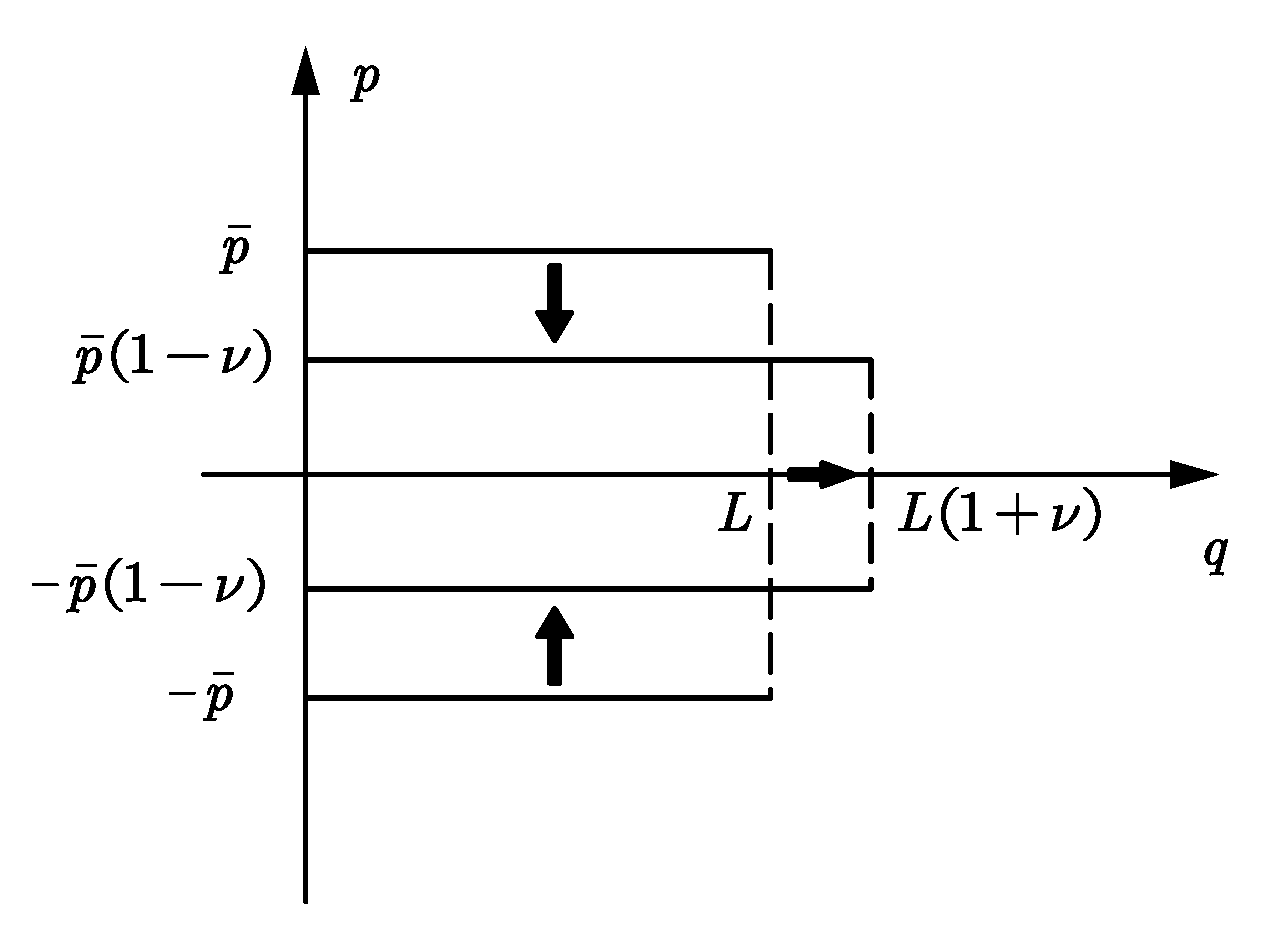
\includegraphics[width=0.5\textwidth]{figures/p2.1.pdf}
    \end{center}
    \caption{在一维盒子中的粒子的能壳。该粒子的能壳是一个矩形,当盒子的长度发生极小的改变时,矩形能壳也发生相应的改变。但矩形的体积不变}
    \label{p2.1}
\end{figure}

系统的哈密顿量为
\begin{equation}
     H_{0}(\bm{\eta} ; L)=\frac{p^{2}}{2 m}+V_{\mathrm{box}}(q ; L)
        \label{eq2.18}
\end{equation}
其中$V_{\mathrm{box}}(q ; L)$代表一维盒子的势场$V_{\mathrm{box}}(q ; L) = \left\{\begin{array}{l} 0 ,\ q<L\\ \infty ,\ q \leq 0\ \text{or}\ q \geq L \end{array}\right.$在经典中这个粒子的运动是平凡的——以相同的速度在两堵墙之间做往返运动。
    
哈密顿量的参数$L$随时间$t$变化,现在我们构造这个系统的\textbf{反绝热哈密顿量}。不难得出,矩形能壳的面积为$I=2 \hat{P} L$,由于矩形能壳的长的变化为$L \to L(1+\nu)$,为了维持矩形能壳的面积,在一阶精度下,可令其宽的微小改变为$2 \hat{P} \to 2 \hat{P} (1-\nu)$,其中$\nu \equiv \delta L / L$。于是,这两个能壳被一个线性放缩所联系
\begin{equation}
    q \rightarrow q(1+\nu) \quad, \quad p \rightarrow p(1-\nu)
    \label{eq2.19}
\end{equation}
现在我们可以通过$(\nu q,\ -\nu p)  = \delta L \{ (q,\ p),\ \xi \}$(式\ref{eq2.15})逆向解出生成元的表达式,于是我们可得一对这样的方程$\left\{ \begin{array}{l} q / L=\partial \xi / \partial p \\ p / L=\partial \xi / \partial q \end{array}\right.$。结合限制条件\ref{eq2.13b},于是可令$\xi = q p / L$。再根据式\ref{eq2.19},我们最终得到
\begin{equation}
    H(\bm{\eta}, t)=H_{0}(\bm{\eta} ; L)+\frac{\dot{L}}{L} q p \quad, \quad L=L(t)
    \label{eq2.20}
\end{equation}
在这个时间依赖的哈密顿量之下,绝热不变量$i(q,\ p;\ L)=2 |p| L$是严格守恒的,不论函数$L(t)$的形式是怎样的。现在我们对于这个具体的例子,实实在在的构造出了\textbf{反绝热哈密顿量},这说明其并不只是存在于形式化理论中,而是可以在实际中加以利用的。

在构造出了经典的\textbf{反绝热哈密顿量}之后,我们也可以通过$\xi$的经典表达式来猜想量子力学中的\textbf{反绝热哈密顿量},因为算符$p,\ q$是不对易的,一个自然的猜想是
\begin{equation}
    \xi(L) = \frac{q p + p q}{2 L}
    \label{eq2.21}
\end{equation}
于是,再联系到已知的量子力学中\textbf{一维无限深势阱}的本征解,非常幸运的,我们发现选择的这个$\xi$满足式\ref{eq2.7}
\begin{equation}
    \left(1+\frac{1}{i \hbar} \delta L \xi \right) \sqrt{\frac{2}{L}} \sin \left(\frac{n \pi q}{L}\right)=\sqrt{\frac{2}{L+\delta L}} \sin \left(\frac{n \pi q}{L+\delta L}\right)
    \label{eq2.22}
\end{equation}
其中的相位由于$A_{n}(L)=i\langle n | \partial_L  n\rangle = 0$而消失。于是可以立刻得到
\begin{equation}
    H(t)=-\frac{\hbar^{2}}{2 m} \frac{\partial^{2}}{\partial q^{2}}+V_{\mathrm{box}}(q ; L)+\frac{\dot{L}}{2 L} \frac{\hbar}{i}\left(q \frac{\partial}{\partial q}+\frac{\partial}{\partial q} q\right)
    \label{eq2.23}
\end{equation}
这样,波函数
\begin{equation}
    \psi_n (q, t)=\sqrt{\frac{2}{L}} \sin \left(\frac{n \pi q}{L}\right) \exp \left(-\frac{i}{\hbar} \int_{0}^{t} \mathrm{~d} t^{\prime} \frac{n^{2} \pi^{2} \hbar^{2}}{2 m L^{2}}\right)
    \label{eq2.24}
\end{equation}
将成为这个哈密顿量的精确解,不论$L(t)$的函数形式如何。




















\section{等温捷径}
    


